\section{Results}\label{sec:results}

\subsection{RQ1: equivalence, backend parity and leaks caused by chunking}\label{sec:equiv}
On every test split the Rust core and the pure-Python reference produced identical predictions (presidio-research 178 spans, secrets 298, RedactionBench 3,167, from the frozen commit). The repository's equivalence suite asserts byte-identical streamed, whole-document and parallel output over exhaustive small chunkings, property-based generated inputs, seam-straddling entities and forced fallbacks, and also checks native parity and declared context; it passed 133 of 133 tests at the final commit. These tests corroborate the theorems for the configurations they exercise; they are not proofs, and they do not exercise the named-entity tier's full input dependence.

\paragraph{How often chunking alone leaks}
The theorems say that chunking cannot add leaks; they do not say how many leaks chunking adds without them. We concatenated each test split into one stream and ran the same pattern pipeline four ways (Table~\ref{tab:chunk}; \texttt{benchmarks/chunking\_leak.py}): \emph{whole}, the reference $\Pi(T)$; \emph{naive}, fixed chunks of $c$ characters; \emph{overlapping windows} of $c + o$ characters advancing by $c$, keeping the detections that start in their own $c$ characters ($o = 256$ and $o = 8192$, the longest declared span); and \emph{SafeStream}, Algorithm~\ref{alg:stream} at its default overlap and $m = w$, over five random chunkings with chunk lengths uniform in $1..2c$. We also ran a dense 4.2\,MB generated log (56,153 gold values) and Loghub's real logs of 16 systems \cite{zhu2023loghub} (4.4\,MB, no redaction labels, so only missed reference detections count).

Naive chunking leaked gold values that the whole-document pass redacts on every corpus: at 1\,KiB, 237 RedactionBench values, 7 on presidio-research, 5 on secrets and 872 in the generated log, and at 64\,KiB still 1 and 12. Overlapping windows removed most of these leaks but not all: at 1\,KiB they still leaked 2 RedactionBench values, 1 presidio-research value and 2 secrets even with $o = 8192$. All seven residual misses come from detectors that read a cue to their left (a key name, a URL-credential prefix, an account label) that lay in the previous window; a longer $o$, which only extends a window to the right, cannot recover them, whereas SafeStream keeps exactly this context as its read-only prefix $P$. On Loghub, naive chunking missed 388 of 18,329 reference detections at 1\,KiB and overlapping windows still missed 3. SafeStream's detection set was identical to the whole-document reference in all 100 pattern-tier runs (five streams, four chunk sizes, five chunkings), and with the spaCy tier on presidio-research, 66 RedactionBench documents, three Loghub systems and all 127 TAB judgments (where naive chunking missed 15 detections at 4\,KiB); for spaCy this is an empirical check, not a proof (Section~\ref{sec:derived}).

\paragraph{The condition applied to someone else's detectors}
Nothing in Eq.~\eqref{eq:wstar} is specific to SafeStream's detectors, so we wrapped another tool's pipeline: Presidio's pattern recognisers, with overlapping spans merged as a redactor masks them, declared bounds $L = 2048$ and $C_{\mathrm{left}} = C_{\mathrm{right}} = 64$ (regex lookarounds read only a few characters), and SafeStream's engine at $w = 2112$ (script \texttt{benchmarks/\allowbreak wrap\_\allowbreak presidio.py}; Online Resource~1, Section~S16). Chunked Presidio leaked as SafeStream's tiers do without the engine: at 1\,KiB, naive chunking left 204 RedactionBench gold values that whole-document Presidio redacts, and overlapping windows still missed up to 1,117 detections even with a 2,112-character overlap. The wrapped engine reproduced whole-document Presidio in every run on presidio-research but in none on RedactionBench or TAB, and the comparison located the cause in a single pattern. Presidio's low-confidence Indian PAN pattern begins with the lookaheads \verb|(?=.*?[a-zA-Z])(?=.*?[0-9]{4})| and is compiled with \texttt{DOTALL}, so a ten-character word is reported whenever four digits appear anywhere later in the text: its right context is unbounded, and no overlap can make chunked output equal whole-document output. With that one pattern removed, the wrapped engine was identical to whole-document Presidio in all 12 runs (three corpora, 1\,KiB and 4\,KiB, two random chunkings), while naive chunking still leaked 145 RedactionBench gold values. The declared bounds are therefore not a property of one implementation: they make an existing detector pipeline safe to stream, and checking them exposes the detectors that cannot be.

\begin{table}[t]
\caption{Leaks caused by chunking alone. Each cell gives missed reference detections / gold spans leaked by chunking (fully redacted by the whole-document pass, not by the variant); Loghub has no gold, so its cells give missed detections only. SafeStream: runs whose detection set is identical to the whole-document reference, out of the random chunkings tried. Overlapping windows keep the detections that start in their own chunk; $o$ is the window overlap in characters. The generated log is synthetic and dense (56,153 gold values in 4.2\,MB). Selected rows; Online Resource~1 (Table~S1) gives every corpus at 1, 4 and 64\,KiB.}\label{tab:chunk}
\footnotesize
\begin{tabular*}{\textwidth}{@{\extracolsep\fill}lrrrl}
\toprule
Corpus (pipeline), chunk $c$ & Naive & $o = 256$ & $o = 8192$ & SafeStream \\
\midrule
secrets (pattern), 1\,KiB & 11 / 5 & 4 / 3 & 2 / 2 & 5 of 5 \\
presidio-research (pattern), 1\,KiB & 5 / 7 & 1 / 1 & 1 / 1 & 5 of 5 \\
RedactionBench (pattern), 1\,KiB & 74 / 237 & 3 / 2 & 3 / 2 & 5 of 5 \\
RedactionBench (pattern), 64\,KiB & 1 / 1 & 0 / 0 & 0 / 0 & 5 of 5 \\
Generated log (pattern), 1\,KiB & 957 / 872 & 0 / 0 & 0 / 0 & 5 of 5 \\
RedactionBench, 66 docs (+spaCy), 4\,KiB & 20 / 10 & 2 / 0 & 2 / 0 & 2 of 2 \\
\midrule
Loghub, 16 real systems (pattern), 1\,KiB & 388 & 3 & 3 & 5 of 5 \\
Loghub, 16 real systems (pattern), 64\,KiB & 9 & 0 & 0 & 5 of 5 \\
Loghub, 3 systems (+spaCy), 4\,KiB & 18 & 4 & 4 & 2 of 2 \\
TAB, 127 judgments (+spaCy), 4\,KiB & 15 / 2 & 3 / 0 & 3 / 0 & 2 of 2 \\
\bottomrule
\end{tabular*}
\end{table}

\subsection{RQ2: memory and throughput}\label{sec:memory}

\begin{figure}[t]
\centering
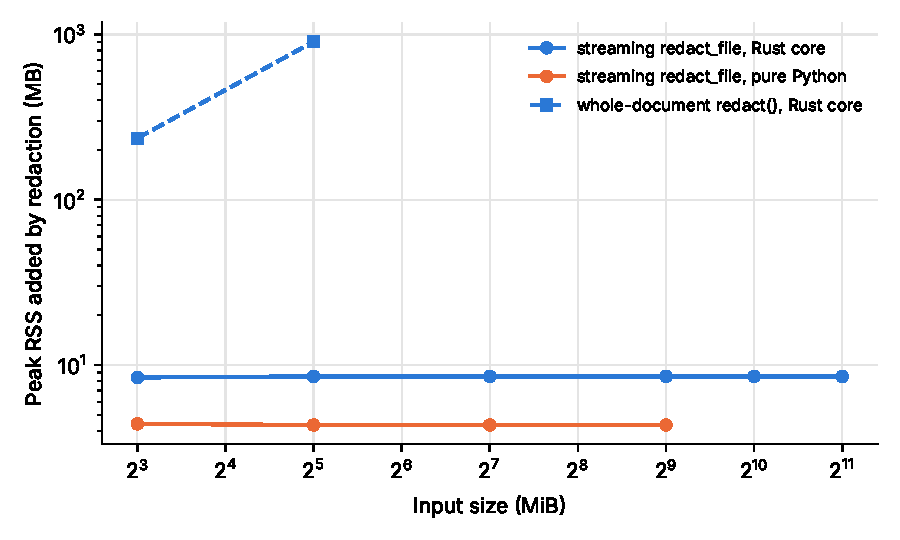
\includegraphics[width=0.7\textwidth]{fig_memory.pdf}
\caption{Peak resident memory added by redaction (peak RSS minus RSS after imports, MiB) against input size, log scales, each point a fresh process. Streaming \texttt{redact\_file} stays flat from 8\,MiB to 2\,GiB (Rust core) and to 512\,MiB (pure Python); whole-document \texttt{redact()} grows with the input.}\label{fig:memory}
\end{figure}

Figure~\ref{fig:memory} plots peak resident memory against input size. Each point is a fresh process redacting a generated log file dense with personal data and credentials. With the Rust core, streaming \texttt{redact\_file} added between 8.4 and 8.54\,MiB at every size from 8\,MiB to 2\,GiB, a 256-fold range. The pure-Python backend added between 4.3 and 4.4\,MiB from 8 to 512\,MiB; it was not run at larger sizes because of its run time (726\,s at 512\,MiB). Whole-document \texttt{redact()} on the same generated inputs, measured the same way, added 235.5\,MiB at 8\,MiB and 904.6\,MiB at 32\,MiB, about 28 times the input size, because the input string, the detections and the output are held at once; at 32\,MiB the two modes therefore differ by a factor of about 106 on identical input. A 128\,MiB whole-document run was stopped after 20 minutes without completing and is not reported. These measurements are consistent with Theorem~\ref{thm:mem} but cover one generated input shape on one machine, and only two whole-document sizes.


On RedactionBench, whose documents average 13.8\,kB, the Rust core processed $10.4 \pm 1.3$\,MB/s with one thread, the pure-Python reference $1.23 \pm 0.15$\,MB/s and Presidio's pattern recognisers 0.069\,MB/s; with a statistical model in the loop every system ran below 0.05\,MB/s. On a 256\,MB generated log, \texttt{redact\_file} with the Rust core ran at $10.5 \pm 0.5$, $20.6 \pm 0.5$ and $41.1 \pm 1.4$\,MB/s with 1, 2 and 4 worker processes, a 3.9-fold speed-up on 4 vCPUs. Online Resource~1 (Table~S2 and Fig.~S1) gives every corpus and system. These figures come from one virtual machine and should be read as relative rather than absolute.

\subsection{RQ3 and RQ4: detection on held-out data}


\begin{table}[t]
\caption{Test-split results with 95\% document-level bootstrap intervals. SafeStream rows are after the entropy fix of Section~\ref{sec:fp}, which changed only the secrets results. FR: fully redacted rate; FA: false-alarm document rate.}\label{tab:main}
\footnotesize
\setlength{\tabcolsep}{3pt}
\begin{tabular*}{\textwidth}{@{\extracolsep\fill}llllll}
\toprule
Corpus / system & Char P & Char R & Char F1 & FR & FA \\
\midrule
\multicolumn{6}{@{}l}{\emph{presidio-research (750 documents)}}\\
SafeStream pattern & \pc{.995}{.992, .998} & \pc{.154}{.133, .176} & \pc{.267}{.235, .299} & \pc{.115}{.098, .134} & .000 \\
SafeStream +dates & \pc{.996}{.993, .998} & \pc{.169}{.146, .192} & \pc{.290}{.255, .322} & \pc{.129}{.110, .150} & .000 \\
SafeStream +spaCy (sm) & \pc{.898}{.877, .918} & \pc{.576}{.547, .606} & \pc{.702}{.679, .725} & \pc{.538}{.509, .568} & .079 \\
Presidio regex & \pc{.948}{.919, .974} & \pc{.175}{.151, .202} & \pc{.296}{.260, .333} & \pc{.123}{.105, .145} & .000 \\
Presidio sm & \pc{.871}{.848, .893} & \pc{.518}{.491, .546} & \pc{.650}{.626, .673} & \pc{.506}{.479, .536} & .048 \\
Presidio lg & \pc{.878}{.856, .900} & \pc{.535}{.507, .563} & \pc{.665}{.642, .688} & \pc{.562}{.534, .590} & .000 \\
\midrule
\multicolumn{6}{@{}l}{\emph{secrets (313 documents)}}\\
SafeStream pattern & \pc{.857}{.705, .946} & \pc{.829}{.740, .887} & \pc{.842}{.736, .906} & \pc{.437}{.384, .498} & .010 \\
SafeStream +spaCy (sm) & \pc{.757}{.604, .858} & \pc{.845}{.762, .897} & \pc{.799}{.683, .870} & \pc{.488}{.435, .548} & .340 \\
gitleaks & \pc{.837}{.630, .962} & \pc{.473}{.299, .679} & \pc{.604}{.430, .765} & \pc{.311}{.253, .375} & .000 \\
TruffleHog & \pc{.803}{.719, .878} & \pc{.189}{.117, .308} & \pc{.306}{.204, .446} & \pc{.270}{.204, .340} & .000 \\
Presidio regex & \pc{.282}{.211, .356} & \pc{.105}{.063, .177} & \pc{.153}{.098, .225} & \pc{.126}{.083, .168} & .392 \\
Presidio sm & \pc{.251}{.191, .315} & \pc{.119}{.072, .197} & \pc{.161}{.107, .232} & \pc{.160}{.112, .206} & .649 \\
Presidio lg & \pc{.308}{.238, .381} & \pc{.131}{.082, .214} & \pc{.184}{.124, .262} & \pc{.164}{.116, .212} & .433 \\
\bottomrule
\end{tabular*}
\end{table}

Table~\ref{tab:main} gives the test-split results (plotted in Online Resource~1, Fig.~S2); The planned differences are tested under clustering in Online Resource~1 (Table~S9).

\paragraph{Credentials (RQ3)}
On secrets, SafeStream's pattern tiers fully redacted 0.437 of test secrets, against 0.311 for gitleaks and 0.270 for TruffleHog (paired document-level differences $+0.128$ [$+0.073$, $+0.183$] and $+0.167$ [$+0.079$, $+0.250$]); precision did not differ significantly. Under resampling by rule (Online Resource~1, Table~S9), the advantage over gitleaks remains in fully redacted rate (two-stage $+0.125$ [$+0.025$, $+0.209$]) and character F1 ($+0.226$ [$+0.011$, $+0.538$]); against TruffleHog only the character-F1 advantage remains ($+0.530$ [$+0.192$, $+0.742$]). SafeStream flagged one of 97 generated non-secrets, neither scanner any. More than half of the test secrets (0.563) were not fully redacted by SafeStream either, mostly vendor formats it has no pattern for; adding spaCy raised its false-alarm rate to 0.340.

\paragraph{Scanner sensitivity}\label{sec:sens}
The gold labels are Nosey Parker's rule examples, and both scanners filter example-like strings, so we re-ran them with their false-positive filters disabled and their rules unchanged (Online Resource~1, Section~S4). gitleaks gained in character F1 (0.604 to 0.805) but little in fully redacted rate (0.311 to 0.328): SafeStream's fully-redacted-rate advantage remains robust ($+0.111$; two-stage [$+0.008$, $+0.193$]), its character-F1 advantage does not survive rule clustering, and TruffleHog changed little. SafeStream's credential patterns were not developed on this corpus; the only change made using it was the suppression rule of Section~\ref{sec:fp}, designed on the development half.

\paragraph{Real credentials (CredData)}
\begin{table}[t]
\caption{Real credentials (CredData): 63,706 labelled line ranges from 337 repositories, values obfuscated by the dataset's builder. FR: fully redacted rate over the 14,626 credential values; FA: share of the 49,517 non-credential ranges with a detection. 95\% intervals under two-stage resampling by repository. SafeStream rows: pattern tiers at the evaluated commit, and the current code's default profile.}\label{tab:cred}
\footnotesize
\setlength{\tabcolsep}{3pt}
\begin{tabular*}{\textwidth}{@{\extracolsep\fill}llllll}
\toprule
System & Char P & Char R & Char F1 & FR & FA \\
\midrule
SafeStream pattern (evaluated) & \pc{.354}{.150, .625} & .817 & \pc{.494}{.249, .720} & \pc{.548}{.313, .739} & \pc{.178}{.100, .271} \\
SafeStream default (current) & \pc{.343}{.146, .634} & .842 & \pc{.487}{.246, .735} & \pc{.717}{.545, .834} & \pc{.328}{.291, .360} \\
gitleaks & \pc{.879}{.714, .945} & .630 & \pc{.734}{.431, .840} & \pc{.398}{.149, .632} & \pc{.023}{.003, .057} \\
TruffleHog & .207 & .004 & .008 & .007 & .006 \\
\bottomrule
\end{tabular*}
\end{table}
The secrets corpus holds rule authors' examples; CredData holds credentials found in real files and labelled by people (Table~\ref{tab:cred}; protocol committed before any run). The planned comparisons show a trade-off rather than a winner. SafeStream's pattern tiers fully redacted more real credentials than gitleaks, 0.548 against 0.398 ($+0.150$ [$+0.142$, $+0.157$]; two-stage by repository $+0.147$ [$+0.085$, $+0.273$]), so the credential-recall margin of the synthetic evaluation holds on real data and survives clustering. They also raised a false alarm on more of the lines that people judged not to hold a credential, 0.178 against 0.023 ($+0.155$; two-stage [$+0.095$, $+0.217$]), and gitleaks' character F1 was higher with lines resampled independently ($-0.237$ [$-0.298$, $-0.185$] for SafeStream) though not robustly so under clustering ([$-0.410$, $+0.011$]). The current code's default profile fully redacted 0.717 of credentials, chiefly because its structured-field tier finds passwords in configuration syntax (fully redacted rate for passwords 0.88, against 0.19 at the evaluated commit and 0.05 for gitleaks), at a false-alarm rate of 0.328. By category, SafeStream led on keys, authorisation headers, URL credentials and nonces, and gitleaks on private keys, tokens and generic secrets (Online Resource~1, Table~S7). TruffleHog redacted almost nothing, plausibly because its detectors key on vendor formats that the shape-preserving obfuscation does not keep; we did not verify this.

\emph{Where the false alarms come from} (descriptive; Online Resource~1, Section~S15). The entropy tier, which supplies most of SafeStream's credential recall, also causes most of its false alarms: without it the pattern tiers fully redacted 0.089 of credentials at a false-alarm rate of 0.075, and 58\% of the flagged non-credential lines carried only entropy-tier detections. SafeStream's confidences do not offer a gitleaks-like operating point: raising the threshold from 0.60 to 0.65 lowers the false-alarm rate to 0.070 but the fully redacted rate to 0.089. CredData's non-credential lines are of two kinds, values judged not to be credentials (\texttt{F}, 45,442 ranges) and test values, examples and placeholders (\texttt{X}, 3,977). The evaluated pattern tiers flagged the two at similar rates (0.178 and 0.167); the current code flagged 0.85 of the \texttt{X} lines, which a redactor that fails closed arguably should mask. The trade-off is a design choice: a redactor that over-redacts loses text, one that under-redacts leaks a secret, while for an alerting scanner the same gap would mean many more alerts to review, which is why gitleaks trades recall for precision. One correction was made after scoring and is disclosed in the protocol: 1,091 ranges labelled as credentials but without a value position had first been counted as non-credential; the protocol counts them as neither, they were removed, and every system's false-alarm rate fell (gold is unchanged).

\paragraph{Personal data (RQ4)}
On presidio-research, the pattern tiers were precise (character precision 0.995) but recalled only 0.154 of sensitive characters, because most gold spans are names, locations and organisations. With the same spaCy model, SafeStream +spaCy exceeded Presidio sm in character F1 by $+0.051$ [$+0.027$, $+0.076$], robust to template clustering (two-stage $+0.052$ [$+0.013$, $+0.093$]); its fully-redacted-rate advantage and its F1 advantage over Presidio lg are not robust. This corpus is synthetic, and Section~\ref{sec:tab} shows that the result does not carry over to real judgments.

\subsection{False alarms on high-entropy non-secrets}\label{sec:fp}

Before the suppression rule of Section~\ref{sec:tiers}, the entropy tier flagged 83 of the 103 generated non-secrets in the development split. The rule, and the secret-key veto that keeps a UUID-shaped access key detected, were designed on the development split. On the test split the false-alarm rate fell from 0.794 [0.714, 0.872] to 0.010 [0.000, 0.035], character precision rose from 0.589 to 0.857, and recall was unchanged. The test half had been scored once with the pre-fix code before the fix was made; both scores are reported. Because the gold-free documents in both halves come from the same generator, the test improvement is an optimistic estimate of the fix's effect on real non-secrets (details in Online Resource~1, Section~S5).

\subsection{RQ5: document-level protection and contamination}\label{sec:contam}

\begin{table}[t]
\caption{RedactionBench test half (100 documents), with 95\% document-level bootstrap intervals. \emph{Exposed}: current code, whose rules were written after inspecting all 200 documents. \emph{Pre-exposure}: the last commit before the benchmark entered the repository. \emph{Dev-selected}: configuration chosen on the development half by a fixed rule (maximum development character F1) and scored on the test half once.}\label{tab:rb}
\footnotesize
\begin{tabular*}{\textwidth}{@{\extracolsep\fill}llll}
\toprule
System & Char F1 & Mandatory recall & No-leak docs \\
\midrule
Pre-exposure, pattern & .518 [.434, .593] & .589 [.476, .696] & .074 [.022, .129] \\
Pre-exposure, +spaCy & .472 [.395, .547] & .674 [.566, .779] & .137 [.073, .208] \\
Pre-exposure, dev-selected & .469 [.394, .543] & .676 [.568, .781] & .137 [.073, .208] \\
Exposed, pattern & .579 [.490, .662] & .682 [.578, .787] & .084 [.032, .144] \\
Exposed, +spaCy & .512 [.429, .590] & .761 [.657, .860] & .179 [.105, .263] \\
Exposed, dev-selected & .508 [.427, .588] & .762 [.658, .862] & .179 [.105, .263] \\
\midrule
gitleaks & .214 [.130, .314] & .247 [.140, .372] & .021 [.000, .053] \\
TruffleHog & .030 [.017, .048] & .024 [.013, .040] & .000 \\
Presidio regex & .323 [.250, .393] & .331 [.227, .422] & .011 [.000, .033] \\
Presidio sm & .336 [.265, .402] & .416 [.326, .500] & .084 [.032, .146] \\
Presidio lg & .344 [.277, .409] & .420 [.333, .499] & .105 [.052, .174] \\
\bottomrule
\end{tabular*}
\end{table}


Table~\ref{tab:rb} separates the contaminated and uncontaminated results. Rules written after inspecting the benchmark raised test mandatory recall of the pattern tiers by $+0.091$ [$+0.044$, $+0.163$] and character F1 by $+0.060$ [$+0.029$, $+0.108$] relative to the pre-exposure code (paired), and both gains are robust to domain clustering. Because those rules were written while the test documents were visible, this gain is an upper bound on what they contribute to unseen data. One of them, the label-anchored tier, also improved presidio-research, a corpus it was never tuned on (Section~\ref{sec:ablation}), which is evidence that it generalises. Development-set selection chose the same configuration for both code versions (spaCy on, entropy on, confidence threshold 0.3).

\paragraph{Pre-exposure code against the baselines}
The pre-exposure code never saw the benchmark, so it gives the uncontaminated comparison (Online Resource~1, Table~S9). With spaCy, its mandatory recall exceeded Presidio lg and sm by $+0.262$ [$+0.091$, $+0.436$] and $+0.265$ [$+0.093$, $+0.441$], robust to domain resampling; its character-F1 advantage is robust against Presidio sm only, and the pattern tiers' F1 advantage over Presidio does not survive domain clustering. Against the secret scanners every pre-exposure configuration was ahead under all three schemes; no-leak rates did not differ significantly from Presidio.

\paragraph{No-leak documents}\label{sec:noleak}
The no-leak document rate was low for every system: at most 0.179 [0.105, 0.263] for SafeStream (+spaCy, exposed code), 0.137 for the pre-exposure code with spaCy, 0.084 for the pattern tiers alone, and at most 0.105 for Presidio. In other words, for at least 82\% of RedactionBench test documents, every configuration we evaluated left at least one must-redact character in the clear. This metric is deliberately strict. Mandatory recall measures the share of must-redact characters hidden; the no-leak rate requires all of them in a document to be hidden, so a single missed character fails the document. RedactionBench documents are dense: the test half averages about 256 gold spans per document (Table~\ref{tab:corpora}), of which 84 on average (median 25) are mandatory.

\emph{Where the leaks are.} Per-document predictions of five systems (Online Resource~1, Section~S6) show that the leaks are whole missed values rather than boundary errors (4.8\% of leaked mandatory characters with spaCy lie in partly redacted spans), that they are concentrated (fixing one or two spans per document would raise the no-leak rate with spaCy only to 0.305), and that they are mostly names without a named-entity model. Even the union of all five systems' redactions would leave 69 of 95 documents leaking (no-leak rate 0.274), so the low document-level rate is a property of the corpus and of current detectors in general, not only of SafeStream. Nor is it caused by streaming: by Theorem~\ref{thm:stream} the streamed output equals the whole-document output, so these leaks are detection misses that a whole-document run would also make.

\subsection{RQ6: detection on real system logs}\label{sec:reallogs}


On real \texttt{sshd} lines (all systems in Online Resource~1, Table~S10), every system with an IP pattern, SafeStream and all three Presidio configurations, redacted all 1,349 IP addresses. No system redacted user names: SafeStream's pattern tiers redacted none of 1,142, and the best configuration, SafeStream with spaCy, redacted 21. User names in phrases such as \texttt{Invalid user webmaster from} carry no shape or label that a pattern tier keys on, and the statistical models rarely tag them. This is the clearest gap that real data exposed. Because user names are nearly half the gold, the fully redacted rate is 0.54--0.55 for every IP-capable system, and only 38--40\% of lines with gold were fully protected.

The systems differed in what else they redacted. Presidio's statistical configurations tagged the syslog timestamp of almost every line as a date and flagged 99--100\% of the lines without gold, against none for SafeStream's pattern tiers, so SafeStream's character F1 exceeded Presidio sm and lg by $+0.291$ and $+0.208$, both robust to template clustering (two-stage [$+0.205$, $+0.351$] and [$+0.130$, $+0.275$]); against Presidio's pattern recognisers the difference ($+0.038$) does not survive clustering. An independent audit of the labels against the values each slot holds (\texttt{benchmarks/\allowbreak loghub\_\allowbreak label\_\allowbreak audit.py}; Online Resource~1, Section~S17) found one defect in how the frozen labels were applied: in 383 lines Loghub's parser leaves a trailing space after the remote address, so the address was not recognised as an IP and was left out of the gold; in another 90 the host is a reverse-DNS name embedding the address, which the rule excludes. Every IP-capable system redacted both, so their precision is understated. With the whitespace handled, character F1 rises for every such system by a similar amount (SafeStream 0.757 to 0.879, Presidio regex 0.719 to 0.838, Presidio lg 0.549 to 0.654), and no comparison changes direction; the frozen labels remain the primary result.

\subsection{A user-name tier for authentication logs}\label{sec:logusers}

In authentication logs a user name is identified not by its shape but by the fixed text the logging program writes around it, so this gap can be closed by rules. We added an opt-in tier (\texttt{use\_log\_usernames}) of 14 patterns anchored on the documented message formats of \texttt{sshd} (\texttt{Invalid user NAME from}), Linux-PAM (\texttt{user=NAME}, \texttt{session opened for user NAME}), \texttt{su}, \texttt{sudo} and \texttt{login}; only the name is redacted, and its declared bounds ($L = 64$, $C_{\mathrm{left}} = 96$, $C_{\mathrm{right}} = 320$) leave $w^{\star}$ at 8192. Because the current default already reads \texttt{user=NAME}, we compare the current code with and without the tier.

\begin{table}[t]
\caption{Held-out real Linux logs (2,000 lines; Loghub). Labels were drafted after the user-name tier was committed and frozen before scoring. IP and user-name columns give the gold values fully redacted by any detection; FA is over the 407 lines without gold. The upper block is the evaluated commit, as in the rest of the paper; the lower block is the current code with and without the user-name tier.}\label{tab:linux}
\footnotesize
\setlength{\tabcolsep}{3pt}
\begin{tabular*}{\textwidth}{@{\extracolsep\fill}lrrrrrr}
\toprule
System & Char P & Char R & Char F1 & IP addresses & User names & FA \\
\midrule
SafeStream pattern & .956 & .866 & .909 & 1,258 / 1,258 & 0 / 618 & .005 \\
SafeStream +spaCy (sm) & .532 & .866 & .659 & 1,258 / 1,258 & 0 / 618 & .452 \\
Presidio regex & .403 & .866 & .550 & 1,258 / 1,258 & 0 / 618 & .251 \\
Presidio sm & .270 & .866 & .412 & 1,258 / 1,258 & 0 / 618 & .526 \\
Presidio lg & .285 & .866 & .429 & 1,258 / 1,258 & 0 / 618 & .686 \\
gitleaks & .000 & .000 & .000 & 0 / 1,258 & 0 / 618 & .000 \\
TruffleHog & .000 & .000 & .000 & 0 / 1,258 & 0 / 618 & .000 \\
\midrule
Current code, default & .959 & .944 & .952 & 1,258 / 1,258 & 372 / 618 & .005 \\
Current code + user-name tier & .961 & 1.000 & .980 & 1,258 / 1,258 & 618 / 618 & .005 \\
\bottomrule
\end{tabular*}
\end{table}

On the held-out Linux logs (Table~\ref{tab:linux}) the tier redacted all 618 user names, every line with gold was fully protected (0.846 without the tier, 0.612 for every IP-capable evaluated configuration), and the false-alarm rate was unchanged. The gain over the current default ($+0.131$ [$+0.115$, $+0.147$] in fully redacted rate) is not robust to template clustering ([$+0.000$, $+0.771$]), because all user names occur in 5 of the 118 templates; against every Presidio configuration the tier's character-F1 advantage is (at least $+0.429$ [$+0.338$, $+0.629$]).

On the OpenSSH lines, whose templates had been read while drafting their labels, the tier redacted 1,127 of 1,142 user names (386 without it); the 15 misses are the literal name \texttt{user} and three names logged after a double space. Both corpora come from two machines, so this is evidence for authentication logs, not for user names in general.

\subsection{RQ7: personal data in real court judgments}\label{sec:tab}


On TAB's test split (full results in Online Resource~1, Tables~S11 and~S5) the evaluated configurations did poorly, reversing the synthetic result of Section~\ref{sec:results}: SafeStream +spaCy had lower character F1 than Presidio sm, $-0.213$ [$-0.243$, $-0.181$], and than Presidio lg, $-0.225$ [$-0.255$, $-0.193$]. Most of the gap is dates, 44.7\% of TAB's gold characters, which Presidio redacted (0.98) and SafeStream's named-entity tier, mapping only person, organisation and place labels, did not (0.01). Direct identifiers, 1,011 person-name and 587 code mentions such as application numbers (\texttt{36110/97}), were rarely protected by any system: entity recall on them was at most 0.077, and in fewer than 1\% of document--annotator pairs was every direct identifier redacted. An entity counts only if all its mentions are redacted, so a name whose title (``Mr'') is left out at one mention is unprotected, and application numbers carry no label or checksum that any evaluated tier keys on. The pattern tiers alone recalled almost nothing (0.004); the secret scanners flagged nothing.

\subsection{A free-text configuration, confirmed on held-out judgments}\label{sec:prose}

The TAB failures have identifiable causes, so we built a configuration for prose and tested it the way the rest of the paper tests rules: designed on development data, frozen, then scored once on data no one had looked at. The protocol, including the systems, metrics and planned comparisons, was committed before any system was run on TAB's development or training split (commit \texttt{f2be354}). TAB's test split had already been seen and is reported only as a secondary, exposed result. The configuration, \texttt{Redactor(profile="prose", use\_ner=True)} at commit \texttt{9c10975}, adds three general mechanisms, all off in the default profile and all within the declared bounds, so $w^{\star}$ stays 8192:
\begin{itemize}
\item the prose profile's date tier, plus bare years, which the date tier does not match;
\item a prose-values tier: sums of money with their currency and number/year references such as case and application numbers (\texttt{47676/99}), each matched on word boundaries;
\item a prose mode of the spaCy tier that keeps a person's title with the name (spaCy leaves out ``Mr'' in ``Mr Eric Oldham'', so the gold mention was only partly redacted) and skips generic institution words such as ``the Court'' or ``Government''.
\end{itemize}
One candidate rule, treating all-capital words as section headings, was tried on the development split and removed because it would also drop acronym organisations, which can identify. No rule names a TAB value.

\begin{table}[t]
\caption{The frozen free-text configuration on held-out data: TAB's training split (1,014 judgments, 1,112 document--annotator pairs), never inspected or scored before the configuration was frozen, and a second genre, Wikipedia biographies (553 summaries, 573 pairs), run with the configuration unchanged. SafeStream free-text: \texttt{profile="prose"} with spaCy, frozen before this run. ER: entity recall, the share of entities all of whose mentions are fully redacted; \emph{Dir.\ prot.}: share of document--annotator pairs in which every direct identifier is fully redacted. 95\% document-level intervals.}\label{tab:prose}
\footnotesize
\setlength{\tabcolsep}{3pt}
\begin{tabular*}{\textwidth}{@{\extracolsep\fill}lrrlllr}
\toprule
System & Char P & Char R & Char F1 & ER direct & ER quasi & Dir.\ prot. \\
\midrule
\multicolumn{7}{@{}l}{\emph{TAB held-out judgments}}\\
SafeStream free-text & .568 & .817 & \pc{.670}{.660, .679} & \pc{.892}{.878, .906} & \pc{.805}{.797, .813} & .787 \\
SafeStream +spaCy (evaluated) & .368 & .360 & \pc{.364}{.353, .374} & \pc{.120}{.107, .134} & \pc{.156}{.150, .163} & .004 \\
Presidio regex & .067 & .038 & \pc{.048}{.044, .052} & \pc{.009}{.005, .014} & \pc{.006}{.005, .007} & .001 \\
Presidio sm & .458 & .625 & \pc{.528}{.519, .537} & \pc{.112}{.099, .127} & \pc{.672}{.661, .683} & .009 \\
Presidio lg & .465 & .641 & \pc{.539}{.530, .548} & \pc{.129}{.113, .144} & \pc{.693}{.682, .703} & .006 \\
\midrule
\multicolumn{7}{@{}l}{\emph{Wikipedia biographies (second genre)}}\\
SafeStream free-text & .827 & .710 & \pc{.764}{.752, .776} & \pc{.660}{.625, .694} & \pc{.617}{.600, .634} & .585 \\
SafeStream +spaCy (evaluated) & .845 & .535 & \pc{.655}{.641, .671} & \pc{.516}{.483, .551} & \pc{.360}{.341, .377} & .494 \\
Presidio regex & .425 & .048 & \pc{.086}{.076, .096} & \pc{.001}{.000, .004} & \pc{.017}{.013, .021} & .000 \\
Presidio sm & .747 & .515 & \pc{.610}{.596, .624} & \pc{.559}{.526, .596} & \pc{.481}{.465, .497} & .461 \\
Presidio lg & .753 & .548 & \pc{.634}{.620, .650} & \pc{.689}{.656, .722} & \pc{.505}{.489, .522} & .618 \\
\bottomrule
\end{tabular*}
\end{table}

On the held-out judgments (Table~\ref{tab:prose}) the free-text configuration was ahead of Presidio lg on every planned comparison: character F1 by $+0.131$ [$+0.122$, $+0.139$], character recall by $+0.177$ [$+0.166$, $+0.187$], entity recall on direct identifiers by $+0.764$ [$+0.744$, $+0.784$] and on quasi identifiers by $+0.112$ [$+0.104$, $+0.122$]. Against Presidio sm every margin was larger (character F1 $+0.141$ [$+0.133$, $+0.149$]). It also had higher precision than either (0.568 against 0.465 for lg). The largest change is in direct identifiers: in 78.7\% of document--annotator pairs every direct identifier was fully redacted, against at most 0.9\% for every other system, because titles now stay with names and application numbers are caught (code recall 0.91 against 0.04 for Presidio lg; by type in Online Resource~1, Table~S6). On the development split the configuration reached character F1 0.742; the held-out value, 0.670, is the one to quote. On TAB's exposed test split it reached 0.732 [0.715, 0.748], against 0.605 for Presidio lg. Its streamed output was identical to its whole-document output on held-out judgments in every chunking tried (941,155 characters, the most spaCy accepts in one call; 4\,KiB and 64\,KiB, two chunkings each), where naive 4\,KiB chunking leaked 22 gold mentions and overlapping windows one.

The configuration was designed on judgments from the same court as that held-out set, so we also ran it, unchanged and under a protocol fixed beforehand, on a second genre: 553 annotated Wikipedia biographies (lower block of Table~\ref{tab:prose}). There it again had higher character F1 than Presidio lg, $+0.129$ [$+0.115$, $+0.144$], higher recall ($+0.162$ [$+0.143$, $+0.182$]), higher precision (0.827 against 0.753) and higher quasi-identifier entity recall ($+0.113$ [$+0.095$, $+0.130$]), and every margin over Presidio sm was positive, direct identifiers included ($+0.101$ [$+0.076$, $+0.127$]). The direct-identifier gain did not carry over against Presidio lg ($-0.029$ [$-0.061$, $+0.004$]): biographies carry no application numbers, and their direct identifiers are names, where the larger spaCy model behind Presidio lg holds its own.

Three limits apply. The configuration has been tested on two genres of formal English prose, not on free text in general. Its precision is moderate: most remaining false alarms are names of courts and states that TAB's annotators did not mark. And one direct identifier in five document--annotator pairs still leaked somewhere, so the configuration reduces exposure substantially without making redacted judgments safe to publish on its strength alone.

\subsection{Ablation}\label{sec:ablation}
An ablation on the test splits (Online Resource~1, Table~S4; document-level intervals, not planned) shows that the entropy tier carried most of the credential recall: without it, character F1 on secrets fell from 0.842 to 0.383 ($+0.455$ [$0.242$, $0.641$]). The label-anchored tier raised character F1 on presidio-research by $+0.030$ [$0.019$, $0.044$], a corpus it was never tuned on. The contextual scorer's own detections changed no result, and the named-entity union rule raised recall by small, mostly significant amounts (at most $+0.013$) at no significant cost in F1 on secrets or RedactionBench.
